\documentclass{beamer}
\usetheme{Pittsburgh}
\usepackage{etex}
\usepackage[setrelation]{math}
\usepackage[modernsign,substopindex,shortmquant,mquantifiertype,
mconnectiveformal,postfixflatinterpret,bracketmodalinterpret,
setfixinterpret,modifopindex,seqinfers,seqoptional,footnotecalculus,abbrseqcontext,shortterms,nosigmaterms,novarterms]{logic}
\usepackage[pretest,nocommandblocks]{progreg}
\usepackage[bracketinterpret,postfixinterpret,bracketmodalinterpret,simplenames]{dL}
\usepackage{tabularx,xcolor,colortbl}
\usepackage{booktabs}
\usepackage{todonotes}
\usepackage{wrapfig}
\usepackage{stmaryrd}
\usepackage{proof}
\usepackage{prettyref}
\usepackage{tikz}
\usepackage{pgfplots}
\usepackage{slidetool}
\usepackage{marvosym}
\usenavigationsymbolstemplate{}
\pgfplotsset{width=8cm,compat=1.9}
 \usetikzlibrary{arrows}
 \usetikzlibrary{calc}
 \usetikzlibrary{fit}
 \usetikzlibrary{positioning,shadows}
 \usetikzlibrary{automata}
 \usetikzlibrary{shapes,arrows}
 \usetikzlibrary{decorations.text}
 \usetikzlibrary{decorations.markings}
 \usetikzlibrary{trees,snakes}
\usetikzlibrary{pgfplots.dateplot}
\usepackage{relsize}
\tikzset{fontscale/.style = {font=\relsize{#1}}}
\usepackage{pgfplotstable}
\usepackage{filecontents}

\definecolor{vermillion}{rgb}{0.8,0.4,0}
\definecolor{myblue}{rgb}{0,0.45,0.7}
\definecolor{myyellow}{rgb}{0.85,0.8,0.17}


\newcommand{\rref}[2][]{\prettyref{#2}}

  \tikzstyle{noteline}=[shorten <=8pt]%
  \tikzstyle{notebox}+=[minimum height=1.1cm]%
\newrefformat{sec}{Section\,\ref{#1}}
\newrefformat{appendix}{Appendix\,\ref{#1}}
 \newrefformat{model}{Model\,\ref{#1}}
 \newrefformat{listing}{Listing\,\ref{#1}}
 \newrefformat{line}{line\,\ref{#1}}
 \newrefformat{def}{Definition\,\ref{#1}}
 \newrefformat{defn}{Definition\,\ref{#1}}
 \newrefformat{thm}{Theorem\,\ref{#1}}
 \newrefformat{ax}{\ref{#1}}
 \newrefformat{prop}{Proposition\,\ref{#1}}
 \newrefformat{lem}{Lemma\,\ref{#1}}
 \newrefformat{cor}{Corollary\,\ref{#1}}
 \newrefformat{ex}{Example\,\ref{#1}}
 \newrefformat{tab}{Table\,\ref{#1}}
 \newrefformat{fig}{Figure\,\ref{#1}}
 \newrefformat{eqn}{(\ref{#1})}
\renewcommand{\ivr}{\psi}
\providecommand{\tweak}[1]{#1}
\newcommand{\untweak}[1]{}
\newcommand{\ignore}[1]{}
\newcommand{\stdI}{\dLint[state=\nu]}%
\newcommand{\ws}{\nu}
\newcommand{\wt}{\omega}%
\newcommand{\I}{\iconcat[state=\ws]{\stdI}}%
\newcommand{\It}{\iconcat[state=\wt]{\stdI}}%
\definecolor{vgray}{rgb}{.35,.35,.35}
\renewcommand*{\irrulename}[1]{\text{\textcolor{vgray}{\upshape#1}}}
\usepackage{tikz}
\usepackage{stmaryrd}
\usetikzlibrary{arrows,matrix}
\newcommand{\isabelle}{Isabelle/HOL\xspace}
\newcommand{\allstate}{\mathcal{S}}
\newcommand{\tvm}{\oslash}
\newcommand{\tvt}{\oplus}
\newcommand{\tvf}{\ominus}
\newcommand{\term}{\mathbf{Term}\xspace}
\newcommand{\lequiv}{\leftrightarrow}
\newcommand{\state}{\mathbf{State}\xspace}
\newcommand{\prop}{\mathbf{Prop}\xspace}
\newcommand{\fml}{\mathbf{Fml}\xspace}
\newcommand{\dLi}{\ensuremath{\dL_{\iota}}\xspace}
\newcommand{\KeY}{KeY}
\newcommand{\tint}[2]{#2\lenvelope#1\renvelope}
\newcommand{\fint}[2]{#2\lenvelope#1\renvelope}
\newcommand{\pint}[1]{\lenvelope#1\renvelope}
\newcommand{\piint}[2]{#2\lenvelope#1\renvelope}
\newcommand{\meps}[2]{\iota{#1}\,{#2}}
\newcommand{\mepsIndef}[2]{\varepsilon{#1}\,{#2}}
\newcommand{\R}{\mathbb{R}}
\newcommand{\err}{\textsf{Err}\xspace}
\newcommand{\ffalse}{\textsf{false}\xspace}
\newcommand{\ftrue}{\textsf{true}\xspace}
\newcommand{\projGen}[2]{\ensuremath{\pi_{#1}}{#2}}
\newcommand{\projL}[1]{\projGen{1}{#1}}
\newcommand{\projR}[1]{\projGen{2}{#1}}
\newcommand{\inR}[1]{\textsf{in}{\ensuremath{\mathbb{R}}}(#1)}
\newcommand{\isT}[1]{\textsf{isT}(#1)}
\newcommand{\om}{\omega}
\newcommand{\tom}{\tilde{\omega}}
\newcommand{\tnu}{\tilde{\nu}}
\newcommand{\tmu}{\tilde{\mu}}
\newcommand{\denote}[1]{\mathsf{E}(#1)}
\newcommand{\llc}[3]{\mathsf{LLC}(#2(#1))}
\newcommand{\cont}[2]{\mathsf{Con}(#2(#1))}
\newcommand{\tder}[2]{\der{#2(#1)}}
\newcommand{\hasdiff}[1]{\mathsf{D}(#1)}
\newcommand{\vepsilon}{\xi}
\newcommand{\bebecomes}{\mathrel{::=}}
\newcommand{\alternative}{~|~}
\newcommand{\ModelPlex}{ModelPlex\xspace}
\providecommand{\KeYmaeraX}{KeYmaera X\xspace}

% CdGL
\newcommand{\GL}{GL}
\newcommand{\CdGL}{CdGL}

\theoremstyle{plain}
\theoremstyle{definition}
\theoremstyle{remark}

\definecolor{semblue}{rgb}{0,0,0.7}
\definecolor{vgreen}{rgb}{.1,.5,0}
\definecolor{vdarkgreen}{rgb}{.06,.3,0}
\definecolor{vred}{rgb}{.7,0,0}
\definecolor{vblue}{rgb}{.1,.15,.62}
\definecolor{vgray}{rgb}{.35,.35,.35}
\definecolor{darkishgray}{rgb}{.35,.35,.35}
\definecolor{vvblue}{rgb}{.14,.21,.868}%{1.4*vblue}
\definecolor{lsblue}{HTML}{16303A}
\definecolor{lslightblue}{HTML}{2E6579}
\definecolor{lsverylightblue}{HTML}{4699B9}
\definecolor{lsgreen}{HTML}{5ECEF9}
\definecolor{lslightgreen}{HTML}{54B9DF}
\definecolor{lsred}{HTML}{B94D5D}
\definecolor{lslightred}{HTML}{F16579}
\definecolor{lsdarkred}{HTML}{3A181D}
\definecolor{smigreen}{RGB}{61,113,120}
\definecolor{smiwhite}{RGB}{221,221,221}
\definecolor{smiblack}{RGB}{25,25,25}
\definecolor{smidarkgray}{RGB}{50,50,50}
\definecolor{smigray}{RGB}{90,90,90}
\definecolor{smired}{RGB}{127,0,0}

\title{Practical, End-to-End Verification for Cyber-Physical Systems}
\author{Brandon Bohrer}
\institute[Thesis Committee] % (optional, but mostly needed)
{
  Andr\'{e} Platzer\\
  Stefan Mitsch\\
  Frank Pfenning\\
  Bradley Schmerl, ISR\\
  Tobias Nipkow, TU Munich
}
\date{Thesis Proposal\\October 25 2019}
\setbeamertemplate{footline}[frame number]
\AtBeginSection[]
{
  \begin{frame}<beamer>{Outline}
    \tableofcontents[currentsection]
  \end{frame}
}
\AtBeginSubsection[]
{
  \begin{frame}<beamer>{Outline}
    \tableofcontents[currentsection,currentsubsection]
  \end{frame}
}

\begin{document}

\begin{frame}
  \titlepage
\end{frame}


\newcommand{\ah}[2]{\action<#1-|alert@#1>{#2}}
\newcommand{\ac}[2]{\action<#1->{#2}}

\section{Motivation}
\begin{frame}[t]{\only<1>{Safety-Critical CPS Need Safety}
\only<2->{Safety-Critical CPS Need Proofs}}
  \begin{center}
    \begin{tabular}{ccc}
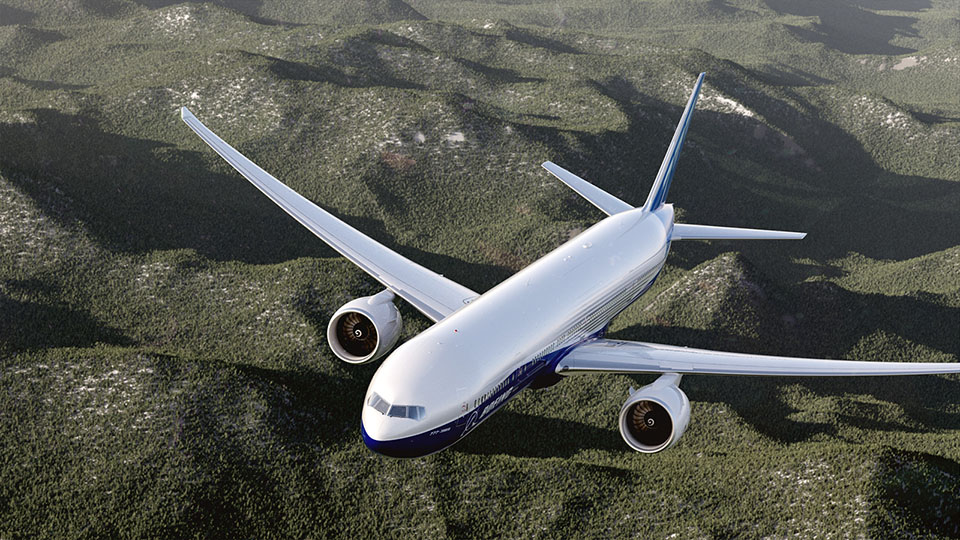
\includegraphics[width=1in]{img/plane-real.jpg}&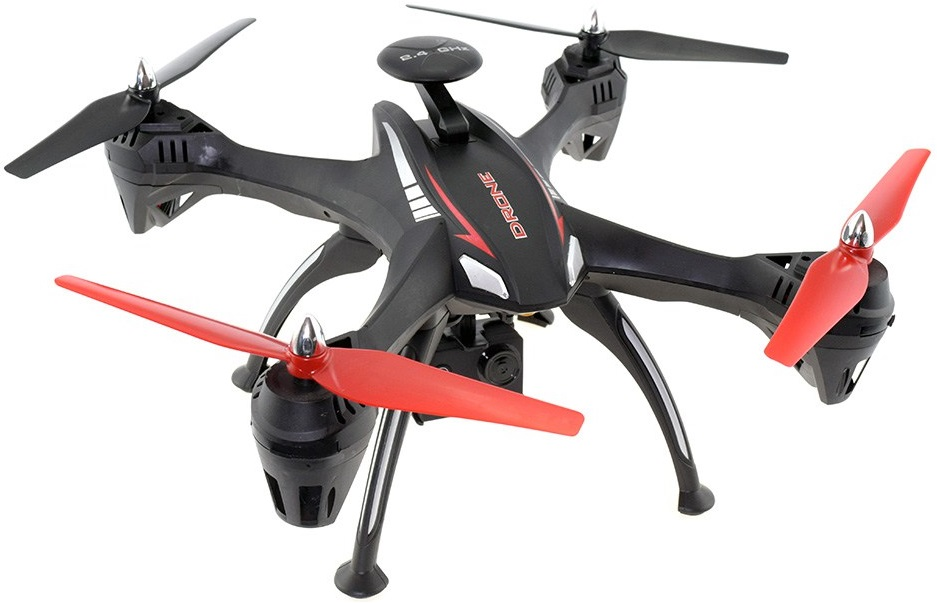
\includegraphics[width=1in]{img/quadcopter-real.jpg}&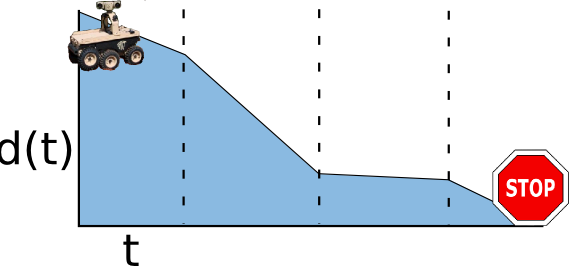
\includegraphics[width=1in]{img/robot-dyn-small.png}\\
Planes&Drones&Robots\\
\uncover<2->{
& &\\
%&$\Downarrow$&\\
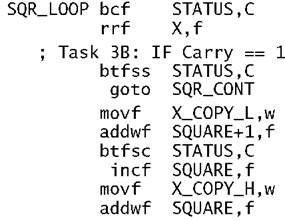
\includegraphics[width=0.6in]{img/assembly-small.png}&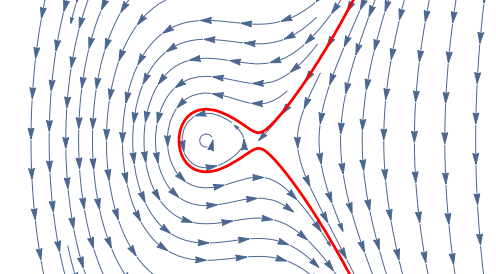
\includegraphics[width=1in]{img/invariant-region.png}&\infer{\Gamma \vdash A \land B}{\Gamma \vdash A}\\
Discrete Control & Continuous Dynamics & Syntactic Proof
}
    \end{tabular}
  \end{center}
  \only<1>{
  \begin{quote}
    How can we design cyber-physical systems people can bet their lives on? -- Jeanette Wing
  \end{quote}
  }
  \only<3>{
  \begin{quote}
    How do proofs cope when control, dynamics are partial, discontinuous?
  \end{quote}
  }
\end{frame}


\begin{frame}[t]{Verification Needs to be End-to-end}
  \begin{tabular}{lll}
%TODO: Make sure all systems are featured in intro pictures
%Pacemaker: 60k, Space shuttle: 400k, car: 100M, F22 > 1M, military drone >3M, 787: 14M, F35: 24M
%codebases
\ah{1}{Application}         & \ah{2}{Models LOC (approx.)}                      & \ah{3}{Real system LOC~\cite{codebases,OpenAPS}} \\
\ac{1}{Insulin pump}        & \ac{2}{30~\cite{COBELLI198227}}                   & \ac{3}{35K}  \\ % number of equations in pape
\ac{1}{Pacemaker}           & \ac{2}{650~\cite{DBLP:conf/cpsweek/AndalamMRT16}} & \ac{3}{60K}  \\ % 35 cells * 19 lines
\ac{1}{Space shuttle}       & \ac{2}{40~\cite{DBLP:conf/cpsweek/ChanM17}}       & \ac{3}{400K}\\ % artifact provided: spaceex
\ac{1}{Modern drone}        & \ac{2}{80~\cite{DBLP:conf/emsoft/RickettsML16}}   & \ac{3}{3M}\\
\ac{1}{Commercial airliner} & \ac{2}{84-150~\cite{DBLP:conf/fm/PlatzerC09,DBLP:conf/emsoft/JeanninGKGSZP15}} & \ac{3}{14M} \\  % tangential roundabout study, safe_explicit.kyx 
\ac{1}{Modern car}          & \ac{2}{29-150~\cite{DBLP:conf/fm/LoosPN11,DBLP:journals/ral/BohrerTMSP19}}  & \ac{3}{100M} %FM kym3 proof, 
  \end{tabular}
\end{frame}

\begin{frame}[t]{End-to-end Verification Must Close Several Gaps}
Why are implementations more complicated than models?
  \begin{align*}
    \text{Learned Controls}   &\rightsquigarrow \text{Control envelopes}\\
    \text{Perception Systems} &\rightsquigarrow \text{Sensing assumptions}\\
    \text{Feedback Controls}  &\rightsquigarrow \text{Actuator assumptions}\\
    \text{Real physics}       &\rightsquigarrow \text{ODE Abstraction}\\
    \text{Non-critical code}  &\rightsquigarrow \langle\textbf{poof}\rangle
  \end{align*}
\end{frame}

\newcommand{\engineer}{
\includegraphics[width=1in]{img/rosie.png}}
\newcommand{\logician}{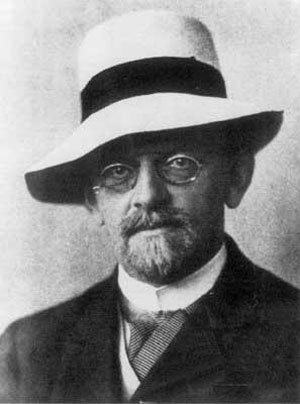
\includegraphics[width=1in]{img/hilbert.png}}
\newcommand{\logicuser}{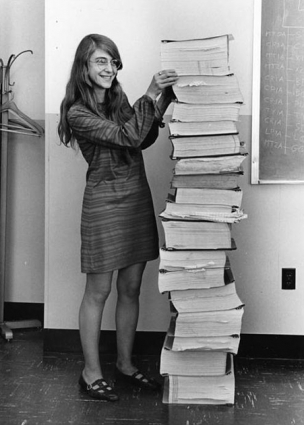
\includegraphics[width=1in]{img/hamilton.png}}

\newcommand{\say}[2]{\small\begin{minipage}{1.3in}{#1}{#2}\end{minipage}}
\newcommand{\sayHappy}[1]{\say{#1}{\Smiley}}
\newcommand{\saySad}[1]{\say{#1}{\Frowny}}

\begin{frame}[t]{End-to-end Verification Must Meet Competing Needs}
  \begin{tabular}{lll}
    \ah{1}{\engineer} & \ah{2}{\logician} & \ah{3}{\logicuser}\\
    \ac{1}{Engineer} & \ac{2}{Logician} & \ac{3}{Logic-User}
  \end{tabular}
\end{frame}

\section{Related Work}
\begin{frame}[t]{General-purpose interactive theorem proving}
  \begin{tabular}{lll}
    \ah{1}{\engineer} & \ah{2}{\logician} & \ah{3}{\logicuser}\\
    \ac{1}{\saySad{Generated code is \\hard to integrate}} & \ac{2}{\sayHappy{Strong Foundations!}} & \ac{3}{\saySad{Long Proofs!}}
  \end{tabular}
  \begin{itemize}
  \item ROSCoq:~\cite{DBLP:conf/itp/AnandK15}       Coq proofs + control synthesis
  \item VeriDrone:~\cite{DBLP:conf/emsoft/RickettsML16}    LTL in Coq + monitor synthesis
  \item Isabelle/UTP:~\cite{DBLP:conf/utp/Foster19} CPS Embedded in Isabelle
  \end{itemize}
% Isabelle/Coq, VeriDrone, ROSCoq
\end{frame}

\begin{frame}[t]{Model Checking + Synthesis}
% LTLMoP, TuLiP, Seshia
  \begin{tabular}{lll}
    \ah{1}{\engineer} & \ah{2}{\logician} & \ah{3}{\logicuser}\\
    \ac{1}{\sayHappy{Synthesis tools!}} & \ac{2}{\saySad{Paper foundations}} & \ac{3}{\saySad{Hard models!}}
  \end{tabular}
  \begin{itemize}
  \item LTLMoP~\cite{DBLP:conf/iros/FinucaneJK10} and TuLiP~\cite{DBLP:conf/IEEEcca/FilippidisDLOM16}: Fancy front-end, synthesis via discretized model
  \item \cite{DBLP:conf/rv/DesaiDS17}: Constant dynamics, STL-based runtime monitor
  \item \cite{DBLP:conf/cdc/BhatiaKV10,DBLP:journals/automatica/FainekosGKP09}: Plan synthesis, complementary to control
  \end{itemize}
\end{frame}

\begin{frame}[t]{\dL Verification + Synthesis (before)}
  \begin{tabular}{lll}
    \ah{1}{\engineer} & \ah{2}{\logician} & \ah{3}{\logicuser}\\
    \ac{1}{\saySad{Limited synthesis}} & \ac{2}{\saySad{Paper foundations}} & \ac{3}{\saySad{Don't like tactics!}}
  \end{tabular}
  \begin{itemize}
  \item Uniform substitution~\cite[\S35,\S40]{Church:1956} is foundation of differential dynamic logic (\dL)~\cite{DBLP:journals/jar/Platzer17}
  \item \KeYmaeraX~\cite{DBLP:conf/cade/FultonMQVP15} prover uses Bellerophon~\cite{DBLP:conf/itp/FultonMBP17} language to express \dL proofs
  \item \ModelPlex~\cite{DBLP:journals/fmsd/MitschP16} synthesizes correct-by-construction monitor conditions from \dL model
  \end{itemize}
% dL, KeYmaera X, ModelPlex
\end{frame}

\begin{frame}[t]{No prior work meets all requirements}
\begin{table}[tbh]
  \centering
\begin{tabular}{l|c|c|r}
Approach    & Logician                 & Engineer                               & Logic-User\\\hline
GPITP       &\cellcolor{green!25}formal &\cellcolor{yellow!25}manual effort      &\cellcolor{orange!25}labor-intensive\\\hline
Automata    &\cellcolor{yellow!25}paper &\cellcolor{green!25}monitors, controls  &\cellcolor{orange!25}error-prone \\\hline
\dL before  &\cellcolor{yellow!25}paper &\cellcolor{yellow!25}some monitors      &\cellcolor{yellow!25}less error-prone\\\hline       %, less labor-intensive
\dL after   &\cellcolor{green!25}formal &\cellcolor{yellow!25}some monitors      &\cellcolor{yellow!25}less error-prone\\\hline\pause %, less labor-intensive
\CdGL       &\cellcolor{green!25}formal &\cellcolor{green!25}monitors, controls  &\cellcolor{green!25}least error-prone\\\hline       %, less labor-intensive
\end{tabular}
  \caption{Comparison of Verification Approaches}
  \label{tab:approach-comparison}
\end{table}
\end{frame}
\begin{frame}[t]{\CdGL Verification + Synthesis (after)}
  \begin{tabular}{lll}
    \ah{1}{\engineer} & \ah{2}{\logician} & \ah{3}{\logicuser}\\
    \ac{1}{\sayHappy{Full synthesis suite!}} & \ac{2}{\sayHappy{Formal foundations!}} & \ac{3}{\sayHappy{Structured proofs!}}
  \end{tabular}
\begin{tabular}{@{\hskip-0.2in}l@{\hskip-0.2in}l}
\begin{minipage}{0.6\textwidth}
{\small\begin{itemize}
  \item[] \textbf{Complete:} Formal soundness proof of \KeYmaeraX core
  \item[] \textbf{Complete:} Verified compilation for \ModelPlex monitors
  \item[] \textbf{Complete:} Logic for discrete games
\end{itemize}}
\end{minipage} &
\begin{minipage}{0.6\textwidth}
{\small\begin{itemize}
  \item[] \textbf{In-progress:} Structured proofs
  \item[] \textbf{Proposed:} Combined monitor, controller synthesis, via
  \item[] \textbf{Proposed:} Logic for hybrid games
\end{itemize}}
\end{minipage}
\end{tabular}

% dL, KeYmaera X, ModelPlex
\end{frame}


\section{Completed Work}

\begin{frame}[t]{Approach of Thesis}
  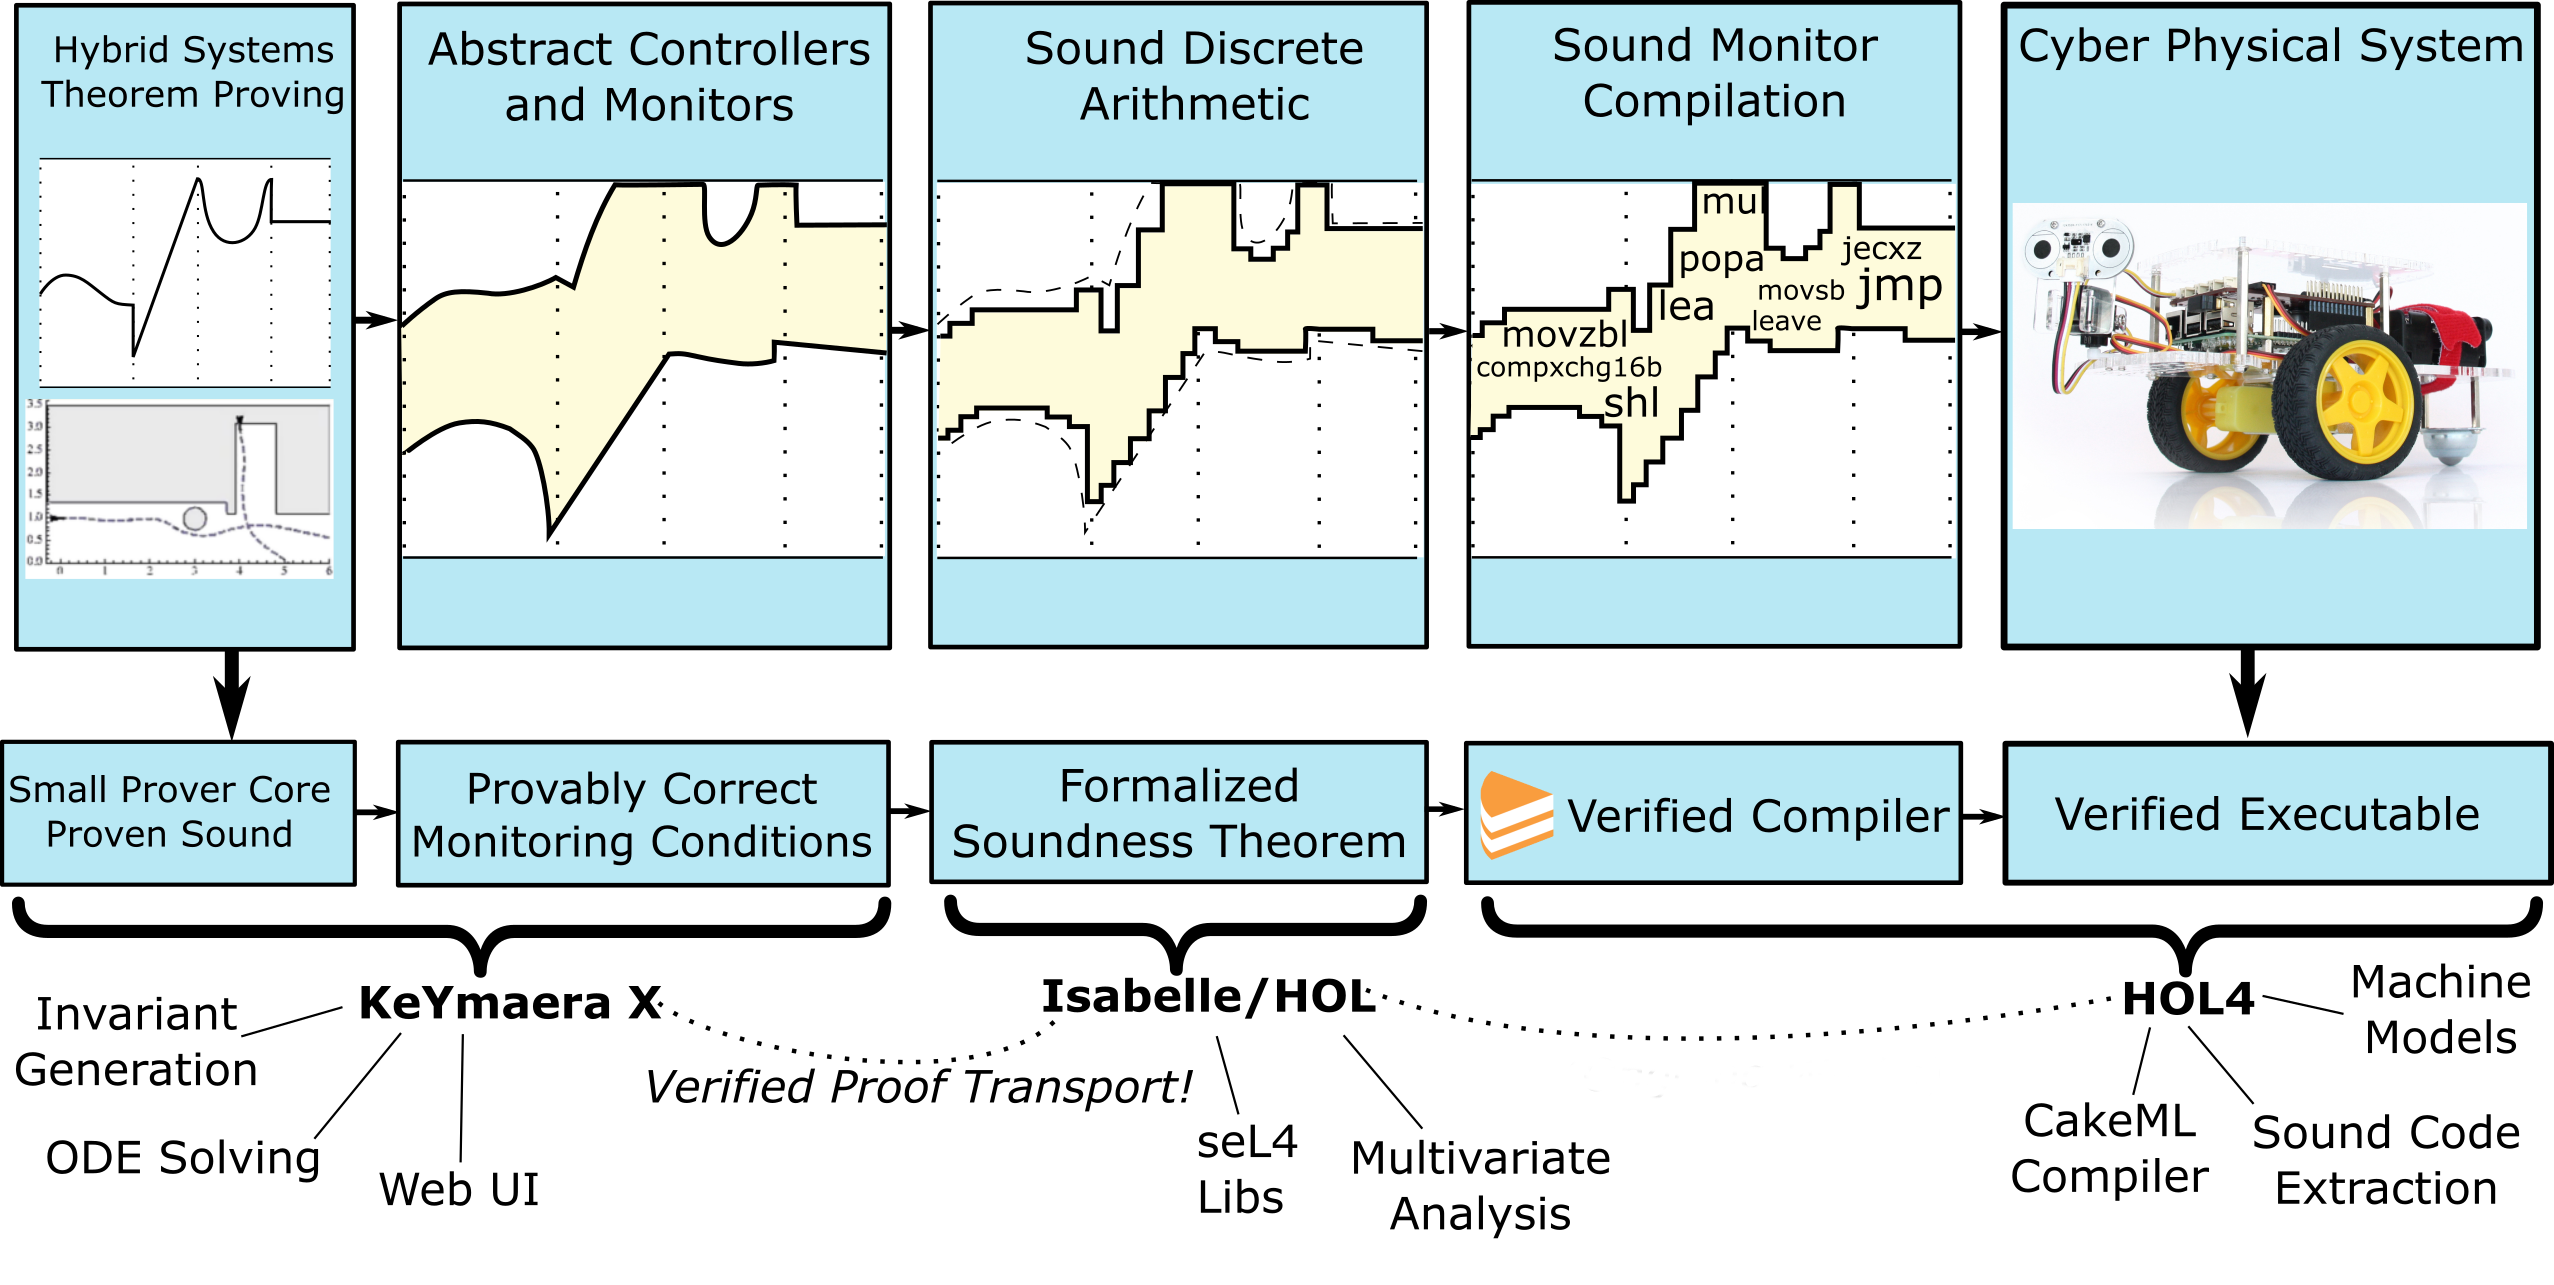
\includegraphics[width=6in]{img/veriphy-overview.png}
\end{frame}

\begin{frame}[t]{Components of Thesis}

\begin{figure}[tbh]
  \centering
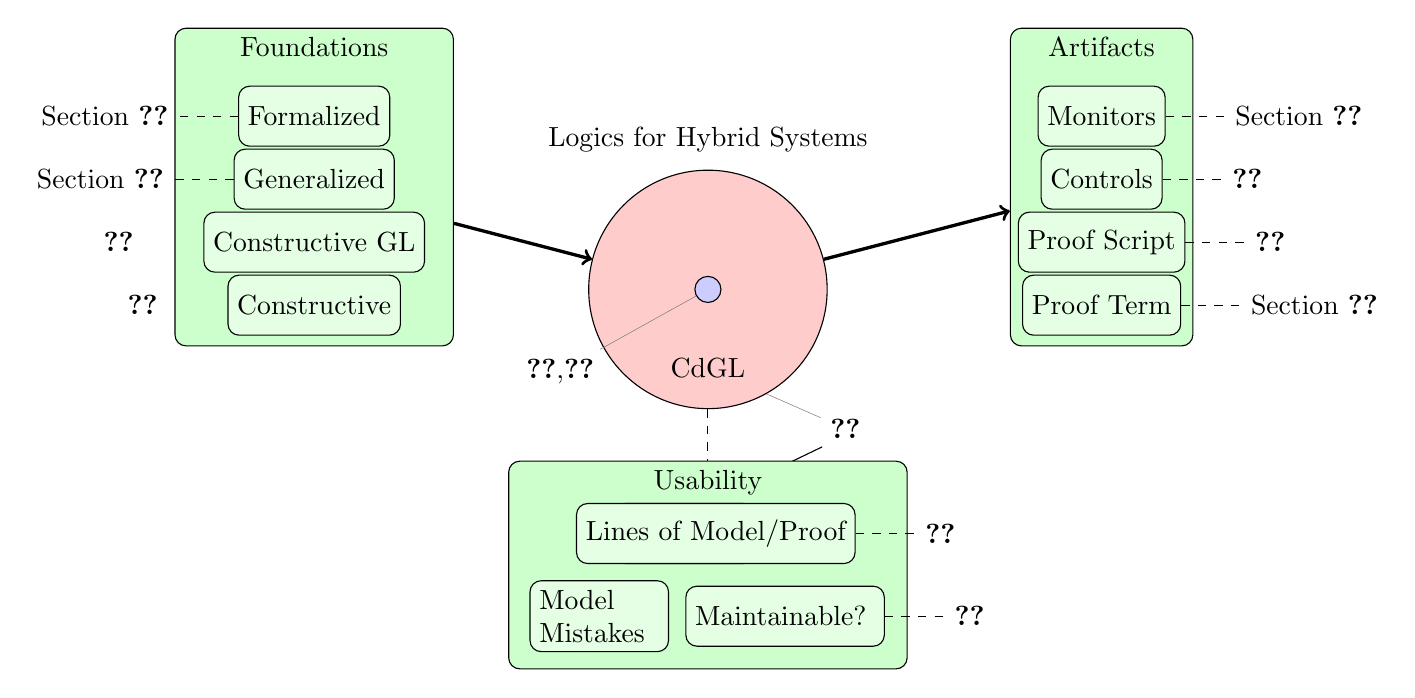
\begin{tikzpicture}
  \draw (0,1.9)  node {Logics for Hybrid Systems};
\draw (0,0)   node[circle]      (CdGLcirc) {\phantom{\hspace{1.1in}}};
\draw (0,-1) node (cdgl) {\phantom{\CdGL}};
\node[coordinate,pin={[pin distance=0.6in]340:{\rref{ch:cdgl}}}] (cdgl-ref) at (cdgl) {};
\draw (0,0)   node[circle, fill=red!20,draw]      (CdGLcirc) {\phantom{\hspace{1.1in}}};
\draw (0,-1) node (cdgl) {\CdGL};
\draw (0,0)   node[circle]  (dl)  {\phantom{\dL}};
\node[coordinate,pin={[pin distance=0.6in]210:{\rref{ch:logical-foundations},\rref{ch:end-to-end-v}}}] (dl-ref) at (dl) {};
\draw (dl) node[circle, fill=blue!20,draw]  {\dL};
\draw (-5, 1.3) node[rectangle,rounded corners,fill=green!20,draw,text depth=1.4in,text width=1.3in,text centered] (logic) {Foundations};
\draw (-5, 2.2) node[rectangle,rounded corners,fill=green!10,draw,thin,minimum height=0.3in] (formalization) {\dL Formalized};
\draw (-5, 1.4) node[rectangle,rounded corners,fill=green!10,draw,thin,minimum height=0.3in] (generalization) {\dL Generalized};
\draw (-5, 0.6) node[rectangle,rounded corners,fill=green!10,draw,thin,minimum height=0.3in] (cgl) {Constructive \GL};
\draw (-5, -0.2) node[rectangle,rounded corners,fill=green!10,draw,thin,minimum height=0.3in] (cdgl) {Constructive \dGL};
\draw node[left=0.3in of formalization] (formal-ref) {\rref{sec:isabelle-fml}};
\draw node[left=0.3in of generalization] (gen-ref) {\rref{sec:definite-description}};
\draw node[left=0.3in of cgl] (cgl-ref) {\rref{ch:cgl}};
\draw node[left=0.3in of cdgl] (cdgl-ref) {\rref{ch:cdgl}};
\draw[dashed] (formalization) -- (formal-ref);
\draw[dashed] (generalization) -- (gen-ref);
\draw (5, 1.3) node[rectangle,rounded corners,fill=green!20,draw,text depth=1.4in,text width=0.82in,text centered] (engine) {Artifacts};
\draw (5, 2.2) node[rectangle,rounded corners,fill=green!10,draw,thin,minimum height=0.3in] (monitors) {Monitors};
\draw (5, 1.4) node[rectangle,rounded corners,fill=green!10,draw,thin,minimum height=0.3in] (controllers) {Controls};
\draw (5, 0.6) node[rectangle,rounded corners,fill=green!10,draw,thin,minimum height=0.3in] (proofscript) {Proof Script};
\draw (5, -0.2) node[rectangle,rounded corners,fill=green!10,draw,thin,minimum height=0.3in] (proofterm) {Proof Term};
\draw node[right=0.3in of monitors] (monitor-ref) {\rref{sec:veriphy}};
\draw node[right=0.3in of controllers] (controllers-ref) {\rref{ch:proofplex}};
\draw node[right=0.3in of proofscript] (proofscript-ref) {\rref{ch:kaisar}};
\draw node[right=0.3in of proofterm] (proofterm-ref) {\rref{sec:veriphy}};
\draw[dashed] (monitors) -- (monitor-ref);
\draw[dashed] (controllers) -- (controllers-ref);
\draw[dashed] (proofscript) -- (proofscript-ref);
\draw[dashed] (proofterm) -- (proofterm-ref);
\node[shape=coordinate] (use-anchor) at (0,-3){};
\draw (1.45,-2) -- (0,-2.7);
\draw (0, -3.5) node[rectangle,rounded corners,fill=green!20,draw,text depth=0.85in,text width=1.9in,text centered] (luser) {Usability};
%\draw (0, -3.1) node[rectangle,rounded corners,fill=green!10,draw,thin,minimum height=0.3in] (monitors)    {Simplicity};
\draw (-0.3, -3.1) node[rectangle,rounded corners,fill=green!10,draw,thin,minimum height=0.3in] (monitors)    {Simplicity};
\draw (0.1, -3.1) node[rectangle,rounded corners,fill=green!10,draw,thin,minimum height=0.3in] (lop)    {Lines of Model/Proof};
%\draw (0, -4.15) node[rectangle,rounded corners,fill=green!10,draw,thin,minimum height=0.3in,text width=0.7in] (controllers) {Modeling Mistakes};
\draw (-1.38, -4.15) node[rectangle,rounded corners,fill=green!10,draw,thin,minimum height=0.3in,text width=0.6in] (modelmistake) {Model Mistakes};
\draw (0.98, -4.15) node[rectangle,rounded corners,fill=green!10,draw,thin,minimum height=0.3in,text width=0.9in] (maintainable) {Maintainable?};
\draw node[right=0.3in of maintainable] (maintain-ref) {\rref{ch:kaisar}};
\draw node[right=0.3in of lop] (lop-ref) {\rref{ch:kaisar}};
\draw[->,very thick] (logic) -- (CdGLcirc);
\draw[->,very thick] (CdGLcirc) -- (engine);
\draw[dashed] (CdGLcirc) -- (luser);
\draw[dashed] (lop) -- (lop-ref);
\draw[dashed] (maintainable) -- (maintain-ref);
\end{tikzpicture}
  \caption{Goals of the thesis}
  \label{fig:goals-diagram}
\end{figure}
\end{frame}
\section{Proposed Work: \CdGL Logic}

\begin{frame}[t]{}
  
\end{frame}

\section{Proposed Work: Kaisar Language}

\begin{frame}[t]{}
  
\end{frame}

\section{Proposed Work: Controller Synthesis}

\begin{frame}[t]{}
  
\end{frame}

\section{Conclusion}
\begin{frame}[t]{}
  
\end{frame}

\appendix
\section<presentation>*{\appendixname}
\subsection<presentation>*{For Further Reading}

\begin{frame}[t, allowframebreaks]
\frametitle{References}
\bibliographystyle{amsalpha}
\bibliography{proposal,platzer,verified-pipeline,hilbert-epsilons,ground-robotics,verified-dL,constructive-games,kaisar}
\end{frame}

\end{document}